\documentclass[a4paper,10pt]{article}
\usepackage[utf8]{inputenc}
\usepackage[T1]{fontenc}
\usepackage[provide=*,french]{babel}
\usepackage{lmodern}
\usepackage[left=0.58cm,right=0.58cm,top=0.40cm,bottom=0.65cm]{geometry}
\usepackage{tikz}
\usepackage{graphicx}
\usepackage{xcolor}
\usepackage{eso-pic}
\usepackage{amssymb,amsmath}
\usetikzlibrary{calc,arrows.meta}
\pagestyle{empty}
\renewcommand{\familydefault}{\sfdefault}
\setlength{\parindent}{0pt}
\renewcommand{\arraystretch}{1.12}

% Couleurs Maths&go
\definecolor{brandNavy}{RGB}{11,53,112}
\definecolor{brandBlue}{RGB}{17,70,140}
\definecolor{brandTeal}{RGB}{29,174,174}
\definecolor{brandOrange}{RGB}{255,145,20}
\definecolor{softBlue}{RGB}{225,238,255}
\definecolor{softTeal}{RGB}{219,247,246}
\definecolor{softOrange}{RGB}{255,238,215}
\definecolor{softGreen}{RGB}{224,246,229}
\definecolor{softGray}{RGB}{245,247,250}
\definecolor{lightLine}{RGB}{190,230,230}

\newcommand{\LogoFile}{../assets/img/mathsgo-logo.png}
\newcommand{\MathsGoFooter}{%
\begin{tikzpicture}[remember picture,overlay]
  \node[anchor=south west,inner sep=0pt] at ([xshift=0.48cm,yshift=0.20cm]current page.south west)
    {\includegraphics[width=2.45cm]{\LogoFile}};
  \node[anchor=west,inner sep=0pt,text=brandNavy,font=\sffamily\bfseries\fontsize{9.2}{10.0}\selectfont]
    at ([xshift=3.16cm,yshift=0.57cm]current page.south west) {mathsgo.re};
\end{tikzpicture}%
}
\AddToShipoutPictureFG{\MathsGoFooter}

% ---------- outils ----------
\newcommand{\LowDotted}[1]{%
\begin{tikzpicture}[baseline=-0.78ex]
  \draw[densely dotted, line width=0.70pt, line cap=round] (0,-0.22) -- (#1,-0.22);
\end{tikzpicture}}
\newcommand{\StepBadge}[1]{\tikz[baseline=-0.62ex]{\node[circle,fill=brandNavy,text=white,font=\bfseries,minimum size=0.54cm,inner sep=0pt]{#1};}}
\newcommand{\StepHead}[2]{\StepBadge{#1}\hspace{0.18cm}{\bfseries\color{brandNavy}\fontsize{12.2}{13.0}\selectfont #2}}
\newcommand{\SubHead}[2]{\textcolor{#1}{\bfseries\fontsize{10.7}{11.4}\selectfont #2}}
\newcommand{\CheckBox}{\ensuremath{\Box}\,}
\newcommand{\Sep}{\vspace{0.05cm}\par\noindent\textcolor{lightLine}{\rule{19.45cm}{0.42pt}}\par\vspace{0.05cm}}
\newcommand{\Apt}{\textcolor{brandOrange}{A}}
\newcommand{\Mpt}{\textcolor{brandBlue}{M}}
\newcommand{\Npt}{\textcolor{brandBlue}{N}}
\newcommand{\Bpt}{\textcolor{brandTeal}{B}}
\newcommand{\Cpt}{\textcolor{brandTeal}{C}}
\newcommand{\AMcol}{\textcolor{brandOrange}{A}\textcolor{brandBlue}{M}}
\newcommand{\ANcol}{\textcolor{brandOrange}{A}\textcolor{brandBlue}{N}}
\newcommand{\ABcol}{\textcolor{brandOrange}{A}\textcolor{brandTeal}{B}}
\newcommand{\ACcol}{\textcolor{brandOrange}{A}\textcolor{brandTeal}{C}}
\newcommand{\BigRatio}[1]{{\fontsize{16.0}{17.0}\selectfont\displaystyle #1}}
\newcommand{\SmallText}[1]{{\fontsize{9.8}{10.5}\selectfont #1}}

\newcommand{\Header}[2]{%
\begin{center}
{\fontsize{22.2}{23.4}\selectfont\bfseries\color{brandNavy} Thalès : démontrer parallèle ou non}\par\vspace{0.02cm}
{\fontsize{13.2}{14.0}\selectfont\bfseries\color{brandTeal} #1}\par\vspace{0.02cm}
{\fontsize{9.9}{10.6}\selectfont\bfseries\color{brandOrange} #2}
\end{center}\vspace{0.02cm}}

% ---------- Figures nettes : pas de bouts arrondis sur les triangles ----------
\newcommand{\FigureEmboitee}[1]{%
\begin{tikzpicture}[scale=#1,line cap=butt,line join=miter]
  \coordinate (A) at (0,0);
  \coordinate (B) at (5.40,-1.20);
  \coordinate (C) at (4.70,2.20);
  \coordinate (M) at (2.59,-0.58);
  \coordinate (N) at (2.26,1.06);
  \fill[softTeal!38] (A)--(B)--(C)--cycle;
  \draw[brandNavy,line width=1.25pt] (A)--(B);
  \draw[brandNavy,line width=1.25pt] (A)--(C);
  \draw[brandTeal,line width=1.38pt] (B)--(C);
  \draw[brandBlue,line width=1.28pt,densely dashed] (M)--(N);
  \foreach \P/\col in {A/brandOrange,M/brandBlue,N/brandBlue,B/brandTeal,C/brandTeal}{\fill[\col] (\P) circle (2.0pt);}
  \node[brandOrange,font=\bfseries\small] at (-0.27,-0.25) {$A$};
  \node[brandBlue,font=\bfseries\small] at (2.62,-0.88) {$M$};
  \node[brandBlue,font=\bfseries\small] at (2.04,1.28) {$N$};
  \node[brandTeal,font=\bfseries\small] at (5.68,-1.18) {$B$};
  \node[brandTeal,font=\bfseries\small] at (4.89,2.42) {$C$};
  \node[brandBlue,font=\bfseries\scriptsize] at (2.83,0.33) {$(MN)$};
  \node[brandTeal,font=\bfseries\scriptsize] at (5.45,0.52) {$(BC)$};
\end{tikzpicture}}

\newcommand{\FigurePapillon}[1]{%
\begin{tikzpicture}[scale=#1,line cap=butt,line join=miter]
  \coordinate (A) at (0,0);
  \coordinate (B) at (3.40,-1.20);
  \coordinate (C) at (2.60,1.90);
  \coordinate (M) at (-2.21,0.78);
  \coordinate (N) at (-1.69,-1.24);
  \draw[brandNavy,line width=1.25pt] (M)--(A)--(B);
  \draw[brandNavy,line width=1.25pt] (N)--(A)--(C);
  \draw[brandBlue,line width=1.28pt,densely dashed] (M)--(N);
  \draw[brandTeal,line width=1.38pt] (B)--(C);
  \foreach \P/\col in {A/brandOrange,M/brandBlue,N/brandBlue,B/brandTeal,C/brandTeal}{\fill[\col] (\P) circle (2.0pt);}
  \node[brandOrange,font=\bfseries\small] at (-0.05,0.31) {$A$};
  \node[brandBlue,font=\bfseries\small] at (-2.50,0.94) {$M$};
  \node[brandBlue,font=\bfseries\small] at (-1.93,-1.43) {$N$};
  \node[brandTeal,font=\bfseries\small] at (3.68,-1.21) {$B$};
  \node[brandTeal,font=\bfseries\small] at (2.80,2.12) {$C$};
  \node[brandBlue,font=\bfseries\scriptsize] at (-2.12,-0.20) {$(MN)$};
  \node[brandTeal,font=\bfseries\scriptsize] at (3.30,0.46) {$(BC)$};
\end{tikzpicture}}

\newcommand{\BlankEmboitee}[1]{%
\begin{tikzpicture}[scale=#1,line cap=butt,line join=miter]
  \coordinate (A) at (0,0);
  \coordinate (B) at (5.40,-1.20);
  \coordinate (C) at (4.70,2.20);
  \coordinate (M) at (2.59,-0.58);
  \coordinate (N) at (2.26,1.06);
  \fill[softTeal!22] (A)--(B)--(C)--cycle;
  \draw[brandNavy!90,line width=1.10pt] (A)--(B);
  \draw[brandNavy!90,line width=1.10pt] (A)--(C);
  \draw[brandTeal,line width=1.18pt] (B)--(C);
  \draw[brandBlue,line width=1.15pt,densely dashed] (M)--(N);
  \foreach \P in {A,M,N,B,C}{\fill[white,draw=brandNavy!60,line width=.70pt] (\P) circle (2.55pt);}
  \node at (-0.36,-0.30) {\LowDotted{0.48}};
  \node at (2.70,-0.88) {\LowDotted{0.48}};
  \node at (2.05,1.30) {\LowDotted{0.48}};
  \node at (5.78,-1.18) {\LowDotted{0.48}};
  \node at (4.96,2.42) {\LowDotted{0.48}};
\end{tikzpicture}}

\newcommand{\BlankPapillon}[1]{%
\begin{tikzpicture}[scale=#1,line cap=butt,line join=miter]
  \coordinate (A) at (0,0);
  \coordinate (B) at (3.40,-1.20);
  \coordinate (C) at (2.60,1.90);
  \coordinate (M) at (-2.21,0.78);
  \coordinate (N) at (-1.69,-1.24);
  \draw[brandNavy!90,line width=1.10pt] (M)--(A)--(B);
  \draw[brandNavy!90,line width=1.10pt] (N)--(A)--(C);
  \draw[brandBlue,line width=1.15pt,densely dashed] (M)--(N);
  \draw[brandTeal,line width=1.18pt] (B)--(C);
  \foreach \P in {A,M,N,B,C}{\fill[white,draw=brandNavy!60,line width=.70pt] (\P) circle (2.55pt);}
  \node at (-0.05,0.34) {\LowDotted{0.48}};
  \node at (-2.53,0.96) {\LowDotted{0.48}};
  \node at (-1.96,-1.45) {\LowDotted{0.48}};
  \node at (3.78,-1.22) {\LowDotted{0.48}};
  \node at (2.87,2.14) {\LowDotted{0.48}};
\end{tikzpicture}}

\begin{document}

% ================= PAGE 1 =================
\Header{Réciproque ou contraposée ?}{Page 1 - méthode guidée avec les lettres données}

\begin{center}
\begin{minipage}[t]{9.35cm}
\centering
\tikz\node[rounded corners=8pt,draw=brandTeal!65,fill=brandTeal!3,line width=0.75pt,text width=8.90cm,inner sep=6pt,align=center]{%
{\bfseries\color{brandTeal} Cas emboîté}\par\vspace{0.02cm}
\FigureEmboitee{0.68}\par\vspace{0.02cm}
{\small $\Apt-\Mpt-\Bpt$ \qquad et \qquad $\Apt-\Npt-\Cpt$}
};
\end{minipage}\hfill
\begin{minipage}[t]{9.35cm}
\centering
\tikz\node[rounded corners=8pt,draw=brandOrange!70,fill=softOrange!25,line width=0.75pt,text width=8.90cm,inner sep=6pt,align=center]{%
{\bfseries\color{brandOrange} Cas papillon}\par\vspace{0.02cm}
\FigurePapillon{0.72}\par\vspace{0.02cm}
{\small $\Mpt-\Apt-\Bpt$ \qquad et \qquad $\Npt-\Apt-\Cpt$}
};
\end{minipage}
\end{center}

\vspace{-0.02cm}
\StepHead{1}{Je vérifie le contexte}\par\vspace{0.05cm}
\begin{center}
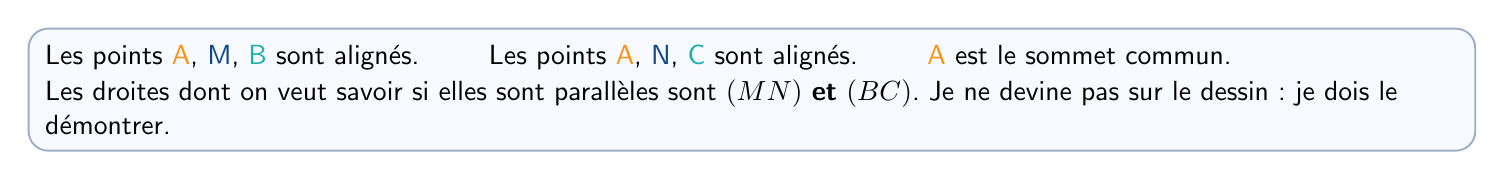
\begin{tikzpicture}
\node[rounded corners=7pt,draw=brandNavy!40,fill=softBlue!28,line width=0.70pt,text width=17.95cm,inner sep=6pt,align=left] {
\SmallText{Les points \Apt, \Mpt, \Bpt{} sont alignés. \hspace{0.65cm} Les points \Apt, \Npt, \Cpt{} sont alignés. \hspace{0.65cm} \Apt{} est le sommet commun.}\par\vspace{0.04cm}
\SmallText{Les droites dont on veut savoir si elles sont parallèles sont \textbf{$(MN)$ et $(BC)$}. Je ne devine pas sur le dessin : je dois le démontrer.}
};
\end{tikzpicture}
\end{center}
\Sep

\StepHead{2}{Je choisis les bons rapports}\par\vspace{0.05cm}
\begin{center}

\begin{tikzpicture}
\node[rounded corners=8pt,draw=brandNavy!35,fill=softGray,line width=0.70pt,text width=17.95cm,inner sep=6.2pt,align=center] {
\begin{minipage}[c]{6.5cm}
\centering
{\bfseries\color{brandTeal} Sur la droite $A,M,B$}\par\vspace{0.02cm}
\fontsize{18}{19}\selectfont $\dfrac{\AMcol}{\ABcol}$
\end{minipage}
\hspace{1.0cm}
\begin{minipage}[c]{6.5cm}
\centering
{\bfseries\color{brandOrange} Sur la droite $A,N,C$}\par\vspace{0.02cm}
\fontsize{18}{19}\selectfont $\dfrac{\ANcol}{\ACcol}$
\end{minipage}
\par\vspace{0.05cm}
{\small\bfseries\color{brandNavy} Même modèle : longueur jusqu'à la droite $(MN)$ / longueur jusqu'à la droite $(BC)$.}
};
\end{tikzpicture}
\end{center}
\Sep

\StepHead{3}{Je calcule les deux rapports}\par\vspace{0.05cm}
\noindent\begin{minipage}[t]{9.50cm}

\begin{tikzpicture}
\node[rounded corners=8pt,draw=brandTeal,fill=brandTeal!5,line width=0.85pt,text width=9.00cm,inner sep=6pt,align=center] {
{\bfseries\color{brandTeal} Premier rapport}\par\vspace{-0.02cm}
\[\BigRatio{\dfrac{\AMcol}{\ABcol}=\dfrac{\LowDotted{0.72}}{\LowDotted{0.72}}=\LowDotted{0.88}}\]
};
\end{tikzpicture}
\end{minipage}\hfill
\begin{minipage}[t]{9.50cm}

\begin{tikzpicture}
\node[rounded corners=8pt,draw=brandOrange,fill=brandOrange!5,line width=0.85pt,text width=9.00cm,inner sep=6pt,align=center] {
{\bfseries\color{brandOrange} Deuxième rapport}\par\vspace{-0.02cm}
\[\BigRatio{\dfrac{\ANcol}{\ACcol}=\dfrac{\LowDotted{0.72}}{\LowDotted{0.72}}=\LowDotted{0.88}}\]
};
\end{tikzpicture}
\end{minipage}

\vspace{0.03cm}
\begin{center}

\begin{tikzpicture}
\node[rounded corners=7pt,draw=brandOrange!55,fill=softOrange!38,line width=0.65pt,text width=17.95cm,inner sep=5pt,align=center] {\textbf{Pour comparer :} je simplifie, je calcule les quotients, ou je fais les produits en croix. Ce n'est pas un tableau de proportionnalité déjà donné : c'est un test.};
\end{tikzpicture}
\end{center}
\Sep

\StepHead{4}{Je compare et je décide}\par\vspace{0.05cm}
\noindent\begin{minipage}[t]{9.50cm}
{\SubHead{brandOrange}{\CheckBox Les rapports sont différents}}\par\vspace{0.04cm}
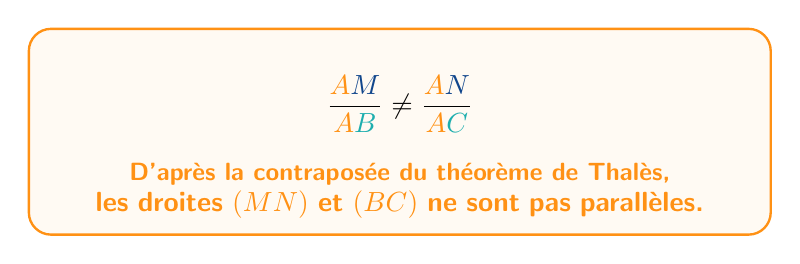
\begin{tikzpicture}
\node[rounded corners=8pt,draw=brandOrange,fill=brandOrange!5,line width=0.85pt,text width=9.00cm,inner sep=6pt,align=center] {
\[\dfrac{\AMcol}{\ABcol}\neq\dfrac{\ANcol}{\ACcol}\]
{\fontsize{9.4}{10.0}\selectfont\bfseries\color{brandOrange} D'après la contraposée du théorème de Thalès,}\par\vspace{-0.03cm}
{\bfseries\color{brandOrange} les droites $(MN)$ et $(BC)$ ne sont pas parallèles.}
};
\end{tikzpicture}
\end{minipage}\hfill
\begin{minipage}[t]{9.50cm}
{\SubHead{brandTeal}{\CheckBox Les rapports sont égaux}}\par\vspace{0.04cm}
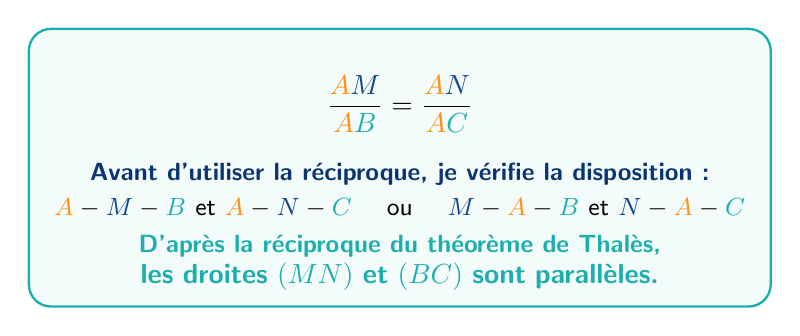
\begin{tikzpicture}
\node[rounded corners=8pt,draw=brandTeal,fill=brandTeal!5,line width=0.85pt,text width=9.00cm,inner sep=6pt,align=center] {
\[\dfrac{\AMcol}{\ABcol}=\dfrac{\ANcol}{\ACcol}\]
{\fontsize{9.3}{10.0}\selectfont\bfseries\color{brandNavy} Avant d'utiliser la réciproque, je vérifie la disposition :}\par\vspace{0.03cm}
{\small $\Apt-\Mpt-\Bpt$ et $\Apt-\Npt-\Cpt$ \quad ou \quad $\Mpt-\Apt-\Bpt$ et $\Npt-\Apt-\Cpt$}\par\vspace{0.04cm}
{\fontsize{9.4}{10.0}\selectfont\bfseries\color{brandTeal} D'après la réciproque du théorème de Thalès,}\par\vspace{-0.03cm}
{\bfseries\color{brandTeal} les droites $(MN)$ et $(BC)$ sont parallèles.}
};
\end{tikzpicture}
\end{minipage}

\vspace{0.08cm}
\StepHead{5}{Je conclus}\par\vspace{0.05cm}
\begin{center}
\tikz[baseline=-0.72ex]{\node[rounded corners=6pt,draw=brandNavy!55,fill=softBlue!18,line width=0.8pt,inner xsep=14pt,inner ysep=6pt,font=\bfseries\fontsize{11.5}{12.2}\selectfont\color{brandNavy}]{Donc les droites $(MN)$ et $(BC)$ sont \LowDotted{3.20}.};}
\hspace{0.4cm}
\tikz[baseline=-0.72ex]{\node[rounded corners=6pt,draw=brandOrange!55,fill=softOrange!35,line width=0.65pt,inner xsep=10pt,inner ysep=5.5pt,font=\bfseries\fontsize{10.0}{10.8}\selectfont\color{brandNavy}]{\CheckBox réciproque \quad \CheckBox contraposée};}
\end{center}

\newpage

% ================= PAGE 2 =================
\Header{Réciproque ou contraposée ?}{Page 2 - gabarit à adapter aux lettres de l'exercice}

\noindent
\begin{minipage}[t]{5.45cm}
\vspace{0pt}
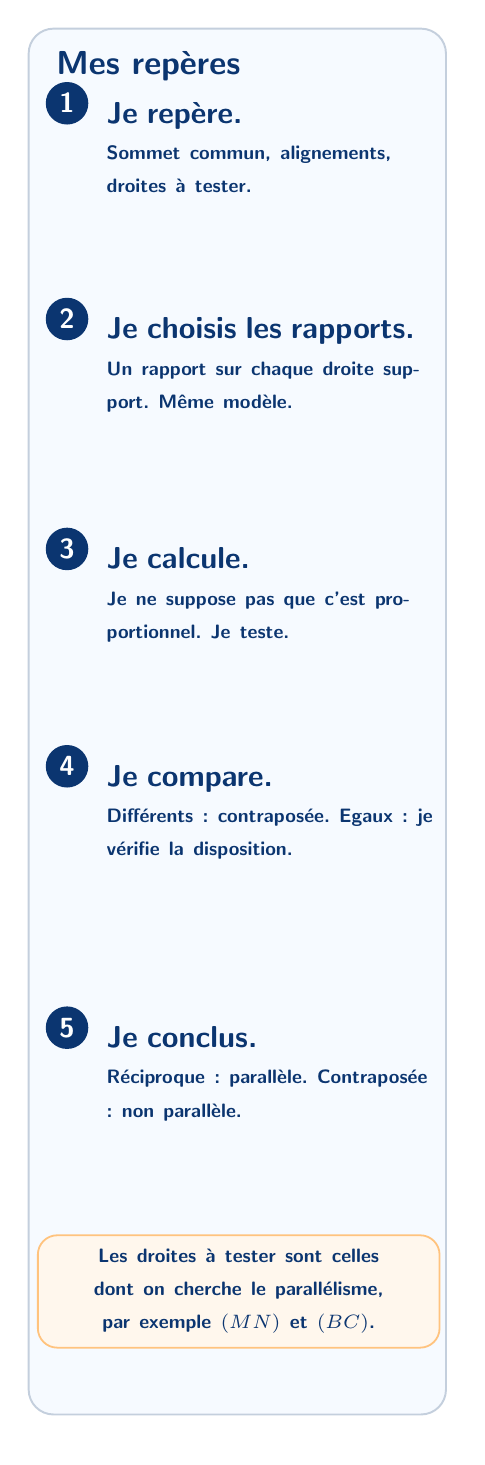
\begin{tikzpicture}[x=1cm,y=1cm]
\path[use as bounding box] (0,0) rectangle (5.45,-17.90);
\node[rounded corners=9pt,draw=brandNavy!24,fill=softBlue!30,line width=0.70pt,minimum width=5.30cm,minimum height=17.60cm,anchor=north west] at (0,0) {};
\node[anchor=north west,text=brandNavy,font=\bfseries\fontsize{12.2}{13.2}\selectfont] at (0.24,-0.18) {Mes repères};

\node[circle,fill=brandNavy,text=white,font=\bfseries,minimum size=0.54cm,inner sep=0pt] at (0.50,-0.96) {1};
\node[anchor=north west,text width=4.15cm,align=left] at (0.88,-0.82) {\bfseries\color{brandNavy}\fontsize{10.6}{11.3}\selectfont Je repère.\par\vspace{0.04cm}
{\scriptsize\bfseries\color{brandNavy} Sommet commun, alignements, droites à tester.}};

\node[circle,fill=brandNavy,text=white,font=\bfseries,minimum size=0.54cm,inner sep=0pt] at (0.50,-3.70) {2};
\node[anchor=north west,text width=4.15cm,align=left] at (0.88,-3.56) {\bfseries\color{brandNavy}\fontsize{10.6}{11.3}\selectfont Je choisis les rapports.\par\vspace{0.04cm}
{\scriptsize\bfseries\color{brandNavy} Un rapport sur chaque droite support. Même modèle.}};

\node[circle,fill=brandNavy,text=white,font=\bfseries,minimum size=0.54cm,inner sep=0pt] at (0.50,-6.62) {3};
\node[anchor=north west,text width=4.15cm,align=left] at (0.88,-6.48) {\bfseries\color{brandNavy}\fontsize{10.6}{11.3}\selectfont Je calcule.\par\vspace{0.04cm}
{\scriptsize\bfseries\color{brandNavy} Je ne suppose pas que c'est proportionnel. Je teste.}};

\node[circle,fill=brandNavy,text=white,font=\bfseries,minimum size=0.54cm,inner sep=0pt] at (0.50,-9.38) {4};
\node[anchor=north west,text width=4.15cm,align=left] at (0.88,-9.24) {\bfseries\color{brandNavy}\fontsize{10.6}{11.3}\selectfont Je compare.\par\vspace{0.04cm}
{\scriptsize\bfseries\color{brandNavy} Différents : contraposée. Egaux : je vérifie la disposition.}};

\node[circle,fill=brandNavy,text=white,font=\bfseries,minimum size=0.54cm,inner sep=0pt] at (0.50,-12.70) {5};
\node[anchor=north west,text width=4.15cm,align=left] at (0.88,-12.56) {\bfseries\color{brandNavy}\fontsize{10.6}{11.3}\selectfont Je conclus.\par\vspace{0.04cm}
{\scriptsize\bfseries\color{brandNavy} Réciproque : parallèle. Contraposée : non parallèle.}};

\node[rounded corners=7pt,draw=brandOrange!55,fill=softOrange!45,line width=0.65pt,text width=4.75cm,inner sep=5pt,align=center] at (2.68,-16.05) {\scriptsize\bfseries\color{brandNavy} Les droites à tester sont celles dont on cherche le parallélisme, par exemple $(MN)$ et $(BC)$.};
\end{tikzpicture}
\end{minipage}\hfill
\begin{minipage}[t]{13.35cm}
\vspace{0pt}

{\bfseries\color{brandTeal}\fontsize{10.8}{11.4}\selectfont J'entoure le cas de l'exercice et je place les lettres sur la figure.}\par\vspace{0.04cm}
\begin{center}
\begin{minipage}[t]{6.35cm}
\centering
\tikz\node[rounded corners=8pt,draw=brandTeal!65,fill=brandTeal!3,line width=0.75pt,text width=5.90cm,inner sep=5pt,align=center]{%
{\bfseries\color{brandTeal}\CheckBox cas emboîté}\par\vspace{0.02cm}
\BlankEmboitee{0.50}
};
\end{minipage}\hfill
\begin{minipage}[t]{6.35cm}
\centering
\tikz\node[rounded corners=8pt,draw=brandOrange!70,fill=softOrange!25,line width=0.75pt,text width=5.90cm,inner sep=5pt,align=center]{%
{\bfseries\color{brandOrange}\CheckBox cas papillon}\par\vspace{0.02cm}
\BlankPapillon{0.55}
};
\end{minipage}
\end{center}

\vspace{0.02cm}
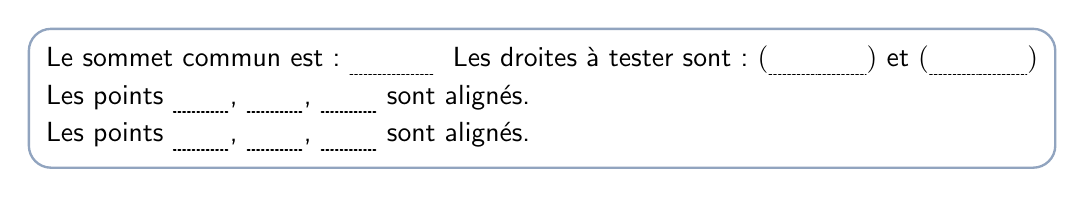
\begin{tikzpicture}
\node[rounded corners=8pt,draw=brandNavy!45,fill=white,line width=0.85pt,text width=12.60cm,inner sep=6.2pt,align=left] {
{\fontsize{10.1}{11.4}\selectfont Le sommet commun est : \LowDotted{1.05}\hfill Les droites à tester sont : $(\LowDotted{0.60}\LowDotted{0.60})$ et $(\LowDotted{0.60}\LowDotted{0.60})$}\par\vspace{0.06cm}
{\fontsize{10.1}{11.4}\selectfont Les points \LowDotted{0.70}, \LowDotted{0.70}, \LowDotted{0.70} sont alignés.}\par\vspace{0.05cm}
{\fontsize{10.1}{11.4}\selectfont Les points \LowDotted{0.70}, \LowDotted{0.70}, \LowDotted{0.70} sont alignés.}
};
\end{tikzpicture}

\vspace{0.08cm}
{\bfseries\color{brandNavy}\fontsize{11.6}{12.4}\selectfont Je choisis puis je calcule les deux rapports}\par\vspace{0.04cm}
\begin{center}
$\begin{array}{rcl}
\BigRatio{\dfrac{\LowDotted{0.82}}{\LowDotted{0.82}}} & = & \BigRatio{\dfrac{\LowDotted{0.76}}{\LowDotted{0.76}}=\LowDotted{0.90}}\\[0.34cm]
\BigRatio{\dfrac{\LowDotted{0.82}}{\LowDotted{0.82}}} & = & \BigRatio{\dfrac{\LowDotted{0.76}}{\LowDotted{0.76}}=\LowDotted{0.90}}
\end{array}$
\end{center}

\vspace{0.04cm}

\begin{tikzpicture}
\node[rounded corners=7pt,draw=brandOrange!55,fill=softOrange!38,line width=0.65pt,text width=12.60cm,inner sep=5.0pt,align=center] {\bfseries\color{brandNavy} Pour comparer : je simplifie, je calcule les quotients, ou je fais les produits en croix.};
\end{tikzpicture}

\vspace{0.10cm}
\noindent\begin{minipage}[t]{6.40cm}
\vspace{0pt}
{\bfseries\color{brandOrange}\fontsize{10.3}{11.0}\selectfont \CheckBox Les rapports sont différents}\par\vspace{0.04cm}
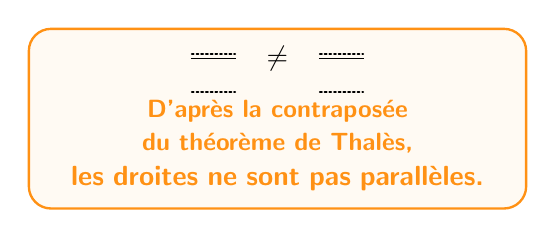
\begin{tikzpicture}
\node[rounded corners=8pt,draw=brandOrange,fill=brandOrange!5,line width=0.85pt,text width=5.88cm,inner sep=6.2pt,align=center] {
$\displaystyle \frac{\LowDotted{0.55}}{\LowDotted{0.55}}\neq\frac{\LowDotted{0.55}}{\LowDotted{0.55}}$\par\vspace{0.05cm}
{\fontsize{9.1}{9.7}\selectfont\bfseries\color{brandOrange} D'après la contraposée du théorème de Thalès,}\par\vspace{0.03cm}
{\bfseries\color{brandOrange} les droites ne sont pas parallèles.}
};
\end{tikzpicture}
\end{minipage}\hfill
\begin{minipage}[t]{6.40cm}
\vspace{0pt}
{\bfseries\color{brandTeal}\fontsize{10.3}{11.0}\selectfont \CheckBox Les rapports sont égaux}\par\vspace{0.04cm}
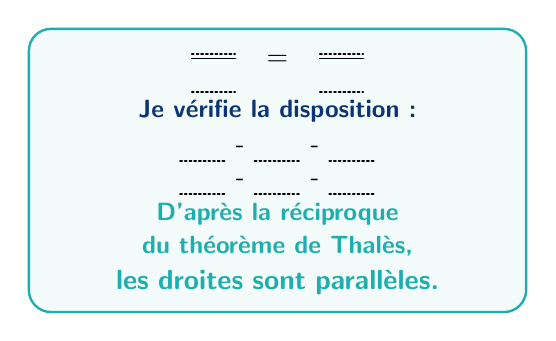
\begin{tikzpicture}
\node[rounded corners=8pt,draw=brandTeal,fill=brandTeal!5,line width=0.85pt,text width=5.88cm,inner sep=6.2pt,align=center] {
$\displaystyle \frac{\LowDotted{0.55}}{\LowDotted{0.55}}=\frac{\LowDotted{0.55}}{\LowDotted{0.55}}$\par\vspace{0.05cm}
{\fontsize{9.1}{9.7}\selectfont\bfseries\color{brandNavy} Je vérifie la disposition :}\par\vspace{0.03cm}
{\small \LowDotted{0.58} - \LowDotted{0.58} - \LowDotted{0.58}}\par\vspace{-0.01cm}
{\small \LowDotted{0.58} - \LowDotted{0.58} - \LowDotted{0.58}}\par\vspace{0.03cm}
{\fontsize{9.0}{9.6}\selectfont\bfseries\color{brandTeal} D'après la réciproque du théorème de Thalès,}\par\vspace{0.03cm}
{\bfseries\color{brandTeal} les droites sont parallèles.}
};
\end{tikzpicture}
\end{minipage}

\vspace{0.18cm}
\begin{center}
\tikz[baseline=-0.72ex]{\node[rounded corners=6pt,draw=brandNavy!55,fill=softBlue!18,line width=0.8pt,inner xsep=12pt,inner ysep=6.2pt,font=\bfseries\fontsize{11.2}{11.9}\selectfont\color{brandNavy}]{Donc les droites $(\LowDotted{0.65}\LowDotted{0.65})$ et $(\LowDotted{0.65}\LowDotted{0.65})$ sont \LowDotted{2.45}.};}
\end{center}

\vspace{0.08cm}
\begin{center}

\begin{tikzpicture}
\node[rounded corners=7pt,draw=brandOrange!55,fill=softOrange!50,line width=0.65pt,text width=12.60cm,inner sep=5.2pt,align=center] {\bfseries\color{brandNavy} Ma réponse est-elle justifiée par le bon mot ? \hspace{0.22cm}$\Box$ réciproque \hspace{0.18cm}$\Box$ contraposée};
\end{tikzpicture}
\end{center}

\end{minipage}
\end{document}
